\placelogofalse
\begin{frame}{Introduction}
\begin{columns}
\column{0.48\linewidth}
\begin{outline}
  \1 Presenting \cite{Hennig2023} (2023)
  \1 Re-architecture of {lbmpy}
  \2 Zero-centered Storage
  \2 Central Moment (CM)
  \2 Cumulants (K)
  \2 Support more generic governing eqns
  \1 Minimizes arithmetic operations for CM and K methods
  \1 Demonstrate small relative cost compared to SRT
\end{outline}
\column{0.48\linewidth}
\begin{center}
  \shadowimage[width=0.46\linewidth]{hennig_paper.png}

  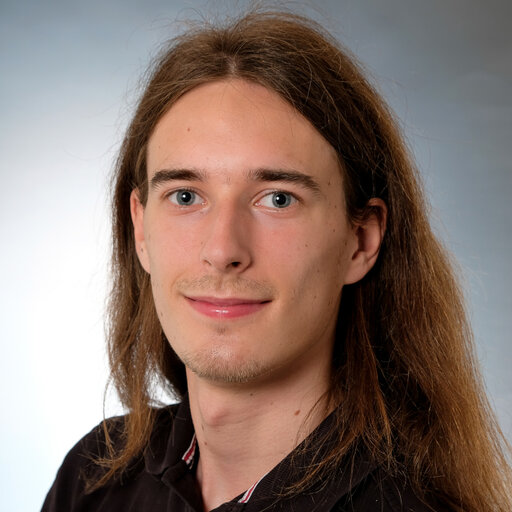
\includegraphics[width=0.28\linewidth]{frederik_hennig.jpg}
  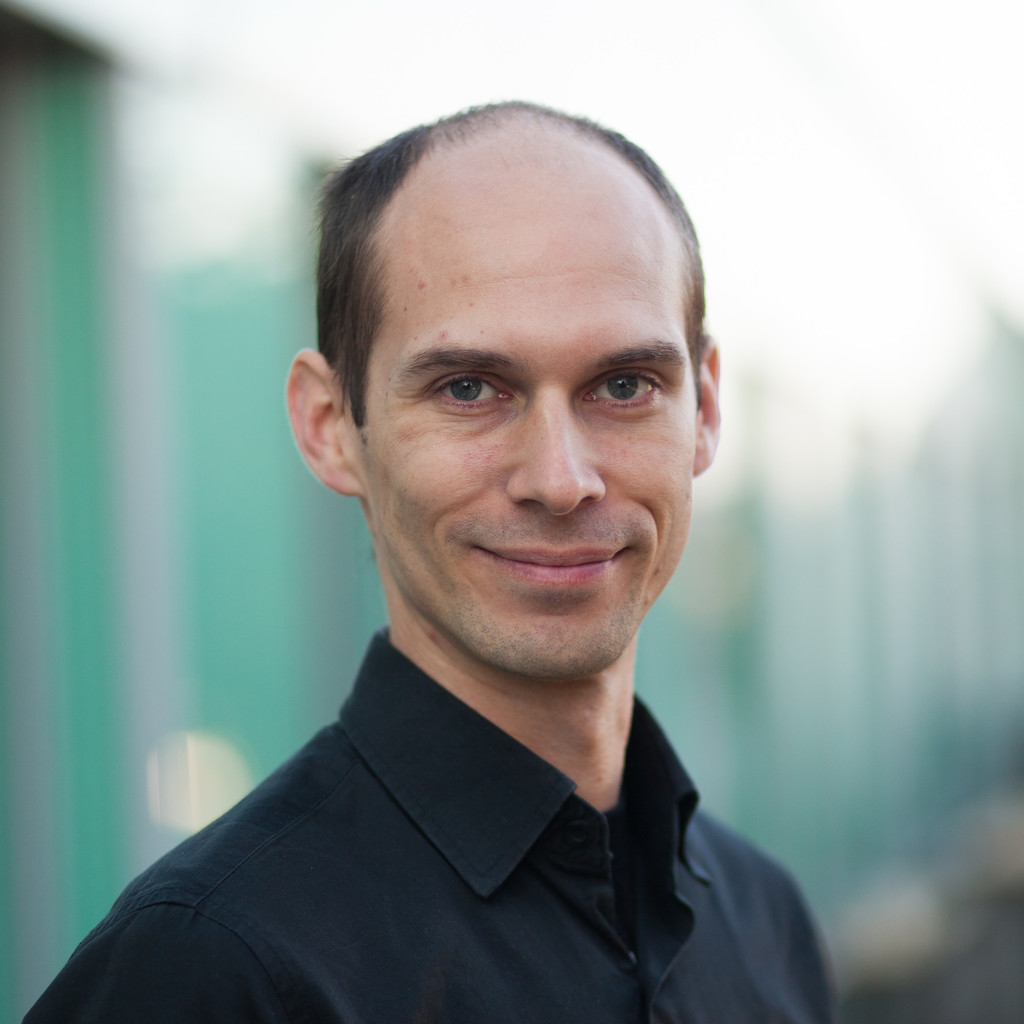
\includegraphics[width=0.28\linewidth]{markus_holzer.jpg}

  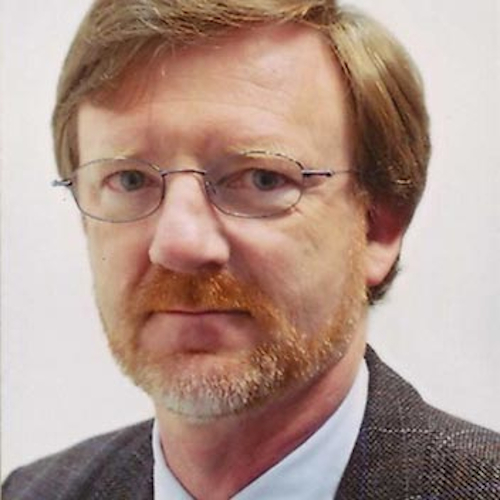
\includegraphics[width=0.28\linewidth]{ulrich_rude.jpg}
\end{center} 
\end{columns}
\end{frame}
\placelogotrue

